\begin{activity} \label{PA:10.13}  In the following questions, we consider two different versions of the Chain Rule.
\ba
\item Figure \ref{F:10.5.tree.2} shows the tree diagram we construct when (a) $z$ depends on $w$, $x$, and $y$, (b) $w$, $x$, and $y$ each depend on $u$ and $v$, and (c) $u$ and $v$ depend on $t$.

\begin{figure}[ht]
  \begin{center}
    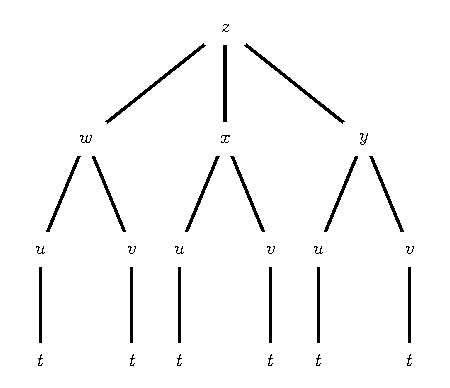
\includegraphics{figures/fig_10_5_tree_2.eps}
  \end{center}
  \caption{Three levels of dependencies}
  \label{F:10.5.tree.2}
\end{figure}

\begin{itemize}
  \item Label the edges with the appropriate derivatives.
  \item Use the Chain Rule to write $\ds\frac{dz}{dt}$.
\end{itemize}

\item Suppose that $T = x^2 + y^2 - 2z$ where
  \begin{align*}
    x & = \rho\sin\phi\cos\theta \\
    y & = \rho\sin\phi\sin\theta \\
    x & = \rho\cos\phi \\
  \end{align*}

  \begin{itemize}
    \item Construct a tree diagram representing the dependencies.
    \item Apply the chain rule to find the partials
      $$
      \frac{\partial T}{\partial\rho},
      \frac{\partial T}{\partial\phi},
      \ 
      \mbox{and}
      \ 
      \frac{\partial T}{\partial\theta},
      \hspace*{20pt}
      $$
    \end{itemize}

  \ea

\end{activity} 
\afterpa 
